%% ─────────────────────────────────────────────────────────────────────────
\subsection{Relevant Context and Motivating Observations}
%% ─────────────────────────────────────────────────────────────────────────

Modern supply chain operators face simultaneous multi-dimensional assessments (cost, deadline, risk, carbon) where most monitoring and planning tools process one criterion at a time~\autocite{pinedo2012scheduling,chakrabortty2020efficient}, which is precisely why practitioners fall back on judgment-based prioritisation.

This work addresses the layer that comes \emph{before} any planning or scheduling decision, and which the classical literature has not fully investigated: the urgency signal itself is systematically biased at the source and must be measured and corrected before it can safely inform any downstream decision~\autocite{zhu2018mere,rusou2020psychology}.

In a Physical Internet network~\autocite{montreuil2011toward}, where logistics capacity is mutualized across actors, a biased urgency signal propagates and amplifies systemic misallocations. Over-triage (declaring an urgency higher than the physical situation warrants) starves other network tenants, whereas under-triage (declaring an urgency lower than warranted) creates invisible stock rupture risk that cascades downstream~\autocite{li2020exploring,ivanov2020digital}.

While digital twin architectures and real-time decision support systems have demonstrated strong capabilities in operational monitoring, disruption detection, resource reallocation, and order synchronisation~\autocite{ding2023realtime,leung2022digital,hrusovsky2021realtime,karam2022realtime,zhu2025industry5}, they do so primarily by computing the physical operational state of the system. To the best of the present review, existing systems do not appear to explicitly model the gap between a declared client urgency and a computed operational urgency.

The core scientific novelty of this R\&D operation therefore lies in the formal comparison between these declared and computed urgencies, propagated coherently across a multi-tier network. This missing integration motivates the introduction of an urgency adequacy layer in digital operations architectures.

\begin{figure}[H]
    \centering
    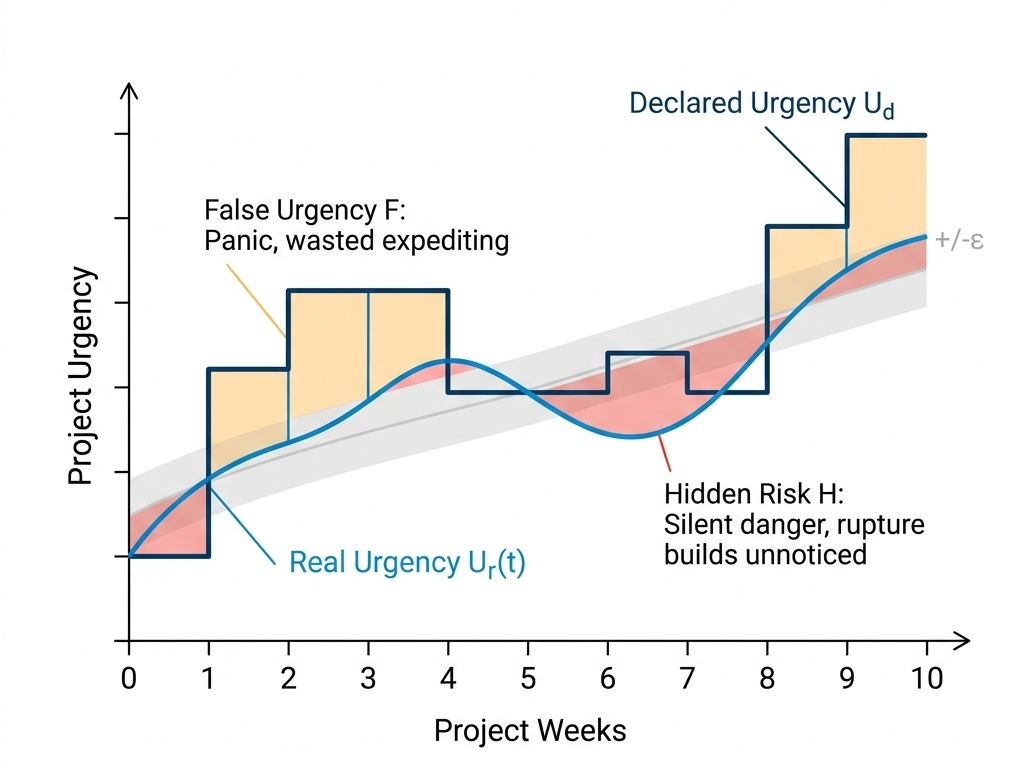
\includegraphics[width=0.85\linewidth]{Images/2.Problem/urgency_gap.png}
    \caption{Conceptual view of the declared vs.\ real urgency gap and its two pathologies. The step line is declared urgency $U_d$ and the smooth curve is real urgency $U_r(t)$; the shaded areas mark where the two mismatch, false urgency $F$ where $U_d$ exceeds $U_r$, hidden risk $H$ where $U_r$ exceeds $U_d$.}
    \label{fig:todraw_gap}
\end{figure}

%% ─────────────────────────────────────────────────────────────────────────
\subsection{Formal Problem Statement}
%% ─────────────────────────────────────────────────────────────────────────

Let $U_d \in [0,1]$ denote the declared urgency and $U_r(t) \in [0,1]$ the real urgency computed from operational data in the digital twin. The core variables and domains are summarized in Table~\ref{tab:problem_vars}.

\begin{table}[H]
\centering
\caption{Core variables and domains.}
\label{tab:problem_vars}
\begin{tabularx}{\linewidth}{lXl}
\toprule
\textbf{Symbol} & \textbf{Meaning} & \textbf{Domain} \\
\midrule
$t$ & Current time (project hours, ISO week granularity) & $\mathbb{R}$ \\
$U_r(t)$ & Physically/operationally computable real urgency & $[0,1]$ \\
$U_d$ & Operator-declared urgency  & $[0,1]$ \\
$\varepsilon$ & Tolerance threshold (cognitive noise band) & $[0,1]$ \\
\bottomrule
\end{tabularx}
\end{table}

The mismatch between both signals is defined as
\begin{equation}
    \Delta U(t) = U_d - U_r(t) \in [-1,\, 1].
    \label{eq:delta_u}
\end{equation}

The components of this mismatch equation are explained in Table~\ref{tab:delta_u_components}.

\begin{table}[H]
\centering
\caption{Component definitions for the urgency discrepancy equation.}
\label{tab:delta_u_components}
\small
\begin{tabularx}{\linewidth}{llX}
\toprule
\textbf{Component} & \textbf{Type} & \textbf{Description} \\
\midrule
$\Delta U(t)$ & Dependent variable & Raw urgency mismatch signal at time $t$ \\
$U_d$         & Input variable     & Urgency level declared subjectively by the human operator \\
$U_r(t)$      & Dynamic variable   & Urgency level computed operationally by the digital twin \\
\bottomrule
\end{tabularx}
\end{table}

A tolerance band $\varepsilon \in [0,1]$ is introduced so that small deviations are not treated as operationally meaningful. In this setting, over-declaration corresponds to $\Delta U(t) > \varepsilon$, under-declaration to $\Delta U(t) < -\varepsilon$, and approximate agreement to $|\Delta U(t)| \le \varepsilon$. Potential consequences of these mismatch conditions are summarized in Table~\ref{tab:pathologies}.

\begin{table}[H]
\centering
\caption{Urgency pathologies and potential consequences.}
\label{tab:pathologies}
\small
\begin{tabularx}{\linewidth}{l >{\raggedright\arraybackslash}X >{\raggedright\arraybackslash}X}
\toprule
\textbf{Condition} & \textbf{Interpretation} & \textbf{Potential consequence} \\
\midrule
$\Delta U(t) > \varepsilon$ & Over-declaration of urgency (false urgency) & Excess expediting, avoidable cost, possible delay for other flows \\[4pt]
$\Delta U(t) < -\varepsilon$ & Under-declaration of urgency (hidden risk) & Hidden lateness or stockout risk, delayed intervention, downstream disruption \\[4pt]
$|\Delta U(t)| \le \varepsilon$ & Acceptable alignment & No material urgency mismatch \\
\bottomrule
\end{tabularx}
\end{table}

An asymmetric treatment of mismatch may be introduced through weights such as $\lambda_{\text{under}} \ge \lambda_{\text{over}}$ when the application context treats under-prioritisation as more harmful than over-prioritisation. This is motivated by operations literature showing that decision errors can generate unequal downstream consequences~\autocite{kim2020admission,diwa2020task}, and by scheduling literature that models differentiated tardiness penalties rather than uniform delay costs~\autocite{baker1982dynamic,chakrabortty2022}. However, the degree of asymmetry is treated here as a design and calibration choice to be validated in the target use case, rather than as a universal property.

%% ─────────────────────────────────────────────────────────────────────────
\subsection{Operation Objectives and Research Questions}
%% ─────────────────────────────────────────────────────────────────────────

The R\&D operation is entitled \textit{``Adequacy Score Between Declared and Real
Urgency in a Smart Green Supply Chain Digital Twin''}. Its three operational objectives are:

\begin{enumerate}[label=\textbf{O\arabic*.}]
    \item Define a multi-block, DAG-propagated real urgency $U_r(t)$ and a cognitive adequacy score $A(t) \in [0, 100]$ to measure the gap between the human planner's declared urgency $U_d$ and the digital twin's operational state.
    \item Develop and implement a network propagation and criticality-driven prioritisation layer, combining PROMETHEE~II outranking with systematic shock simulation, to identify structurally critical nodes.
    \item Validate the adequacy-driven prioritisation logic empirically, through worked scenarios and a calibration service comparing the hidden-risk signal against recorded operational outcomes.
\end{enumerate}

Four research questions structure the scientific approach to these objectives:

\begin{enumerate}[label=\textbf{RQ\arabic*}., leftmargin=*]
  \item \textbf{Multi-block real urgency ($U_r(t)$):}
  How can a physically and operationally grounded real urgency $U_r(t)$ be computed dynamically in a multi-tenant digital twin from heterogeneous KPI blocks (temporal, capacity, performance, risk, cost, environmental), and propagated coherently across a multi-tier supply chain graph?

  \item \textbf{Cognitive adequacy formulation ($A(t)$):}
  How should an adequacy score $A(t)$ be formulated to measure the alignment between operator declared urgency $U_d$ and computed real urgency $U_r(t)$, while asymmetrically penalizing under-triage vs.\ over-triage, and can this scoring demonstrate predictive validity against real operational outcomes?

  \item \textbf{Network prioritisation and criticality:}
  How can pairwise elicitation methods (AHP, Fuzzy Best-Worst Method) be combined with outranking aggregation (PROMETHEE~II) and systematic shock simulation to identify which nodes of a supply network are structurally critical and warrant prioritised attention?

  \item \textbf{Operational validation within a digital twin:}
  How can this cognitive-physical framework be operationalised and empirically validated within a persistent, multi-tenant digital twin exercised as a weekly-cadence serious game, and what predictive validity does it demonstrate against recorded operational incidents?
\end{enumerate}

%% ─────────────────────────────────────────────────────────────────────────
\subsection{Research Hypotheses}
\label{sec:hypotheses}
%% ─────────────────────────────────────────────────────────────────────────

These hypotheses apply to the entire study. They are formulated here, once, so that the evaluation criteria are fixed before any method is introduced, and they match the pre-registered hypothesis register of the validation campaign described in Section~\ref{sec:serious_game}. Each is falsifiable: it states an observable outcome, with a numeric threshold, that the delivered system either does or does not exhibit.

\begin{description}
    \item[H1 (Cognitive latency):] Declared urgency follows computed real urgency with a delay of at least one weekly cycle on the majority of nodes: operators register a degradation after the physical signal, not with it. Test: the lagged correlation between $U_d$ and $U_r$ peaks at a lag of one week or more for at least five of the eight campaign nodes.
    \item[H2 (Early detection of hidden risk):] The hidden-risk signal $H = \max(U_r - U_d, 0)$ exceeds $0.3$ at the crisis-origin node several weeks before the rupture becomes publicly visible.
    \item[H3 (Structural criticality):] The systematic shock simulation ranks the true crisis origin first, by impact on the final customer, among deep-tier suppliers, on at least 80\% of the informative (non-saturated) weekly rounds.
    \item[H4 (Predictive validity):] At threshold $H \ge 0.5$ with a four-week horizon, the hidden-risk signal predicts recorded negative outcomes (missed milestone, critical event, node abandonment) with precision and recall both above $0.5$.
    \item[H5 (Urgency contagion):] On weeks when crisis news becomes public, operators of nodes that are not physically affected still raise their declared urgency, reproducing the mere-urgency effect~\autocite{zhu2018mere} at network scale.
    \item[H6 (Perception hysteresis):] Once the physical situation improves, declared urgency decays at less than half the rate of real urgency: panic outlives its cause.
\end{description}

If H1 and H5 fail, operators need no debiasing and the adequacy layer is redundant. If H2 and H4 fail, the hidden-risk signal is a descriptive curiosity rather than a decision aid. If H3 fails, network prioritisation cannot be trusted operationally. If H6 fails, over-declaration is self-correcting and the asymmetric penalty needs recalibration.

\paragraph{Model Assumptions.}
Distinct from these testable hypotheses, the framework rests on a set of stated modelling assumptions, each verifiable in the delivered code: the network is a directed acyclic graph (no feedback loops, linear topological sort); reviews follow a strict ISO weekly cycle; declared urgency is damped as it descends toward suppliers while real risk is amplified as it ascends toward the customer, each scaled by a per-arc coefficient; the six KPI blocks are treated as independent to permit a probabilistic aggregation; task statuses drive explicit override rules; and the cognitive loss is deliberately asymmetric, with under-declaration priced at roughly twice the cost of panic. These assumptions are design commitments, not empirical claims; the limitations they induce are catalogued in Section~\ref{sec:limitations}.

%% ─────────────────────────────────────────────────────────────────────────
\subsection{Technical and Scientific Challenges}
\label{sec:locks}
%% ─────────────────────────────────────────────────────────────────────────

To evaluate the validity of the proposed framework, its performance is investigated against five scientific challenges identified in contemporary literature. Each challenge is stated here as an open problem; the design choices made to overcome them are in Section~\ref{sec:Operations}.

\begin{attentionBox}
\noindent\textbf{Challenge~1: Justifying the Urgency Aggregation}

\smallskip
Real urgency can be modeled from a single deadline-proximity signal or from an aggregation of heterogeneous risk blocks (slack, capacity saturation, performance, failure exposure, cost drift, emissions overshoot). A single-block, purely time-driven curve is analytically convenient but discards information available in a live digital twin. Conversely, any multi-block aggregation rule must be theoretically justified against simpler linear or averaging alternatives~\autocite{cheng1992scheduling,cheng1996due,cheng2025survey,miller2010}: which rule preserves the visibility of a single catastrophic indicator without letting noise dominate, and on what grounds?
\end{attentionBox}

\begin{attentionBox}
\noindent\textbf{Challenge~2: Reliability of Declared Urgency}

\smallskip
Eliciting the declared urgency $U_d$ via pairwise multi-criteria methods introduces cognitive noise and ranking instability. These methods are sensitive to human inconsistency and rank reversal, meaning that declared urgency cannot be assumed as a deterministic ground truth~\autocite{afrasiabi2022extended,triantaphyllou2024,liang2020}. Operator judgments must therefore be treated as noisy, stochastic inputs~\autocite{stam1997}: how can an elicitation protocol detect and reject inconsistent judgments before they contaminate the network state?
\end{attentionBox}

\begin{attentionBox}
\noindent\textbf{Challenge~3: Value-Added of the Adequacy Signal}

\smallskip
Computing $\Delta U(t) = U_d - U_r(t)$ is necessary but not sufficient. The decisive scientific test is whether this adequacy signal improves the identification of operationally at-risk nodes beyond the raw variables already available to an operator (local KPI thresholds, unweighted urgency, or simple node degree)~\autocite{cohen2021assigning,bojarski2021}. If the score does not demonstrably outperform these simpler baselines against recorded outcomes, it serves merely as an auxiliary decision metric rather than a primary planning signal~\autocite{ahmetoglu2025,turner2021}.
\end{attentionBox}

\begin{attentionBox}
\noindent\textbf{Challenge~4: Composite Score Interpretability}

\smallskip
Aggregating multiple criteria into a single composite score, whether the local urgency $U_r$ across six KPI blocks or a ranking across a network of nodes, risks obscuring trade-offs and weakening decision interpretability. Composite-index literature warns that nominal weights do not always reflect real influence due to component correlations~\autocite{greco2018,becker2017,borgonovo2021global}: how can a coordinator still see \emph{which} indicator is driving a node's urgency once everything is folded into one number?
\end{attentionBox}

\begin{attentionBox}
\noindent\textbf{Challenge~5: No Precedent for Urgency Adequacy}

\smallskip
Digital twin systems routinely monitor real-time operational states, disruption responses, and order synchronization~\autocite{ding2023realtime,leung2022digital,Zha21,Zha26b,Zho21c}. However, to the best of our knowledge, no existing digital twin or decision support system simultaneously captures a client-declared urgency signal, computes a model-based operational urgency from live system state, and measures their mismatch as an active, network-propagated indicator. The absence of precedent cuts both ways: it signals an opportunity, but it also means there is no established architecture, calibration practice, or evaluation benchmark to build on~\autocite{zheng2022,niloofar2023,kalaboukas2021}.
\end{attentionBox}

\begin{figure}[H]
    \centering
    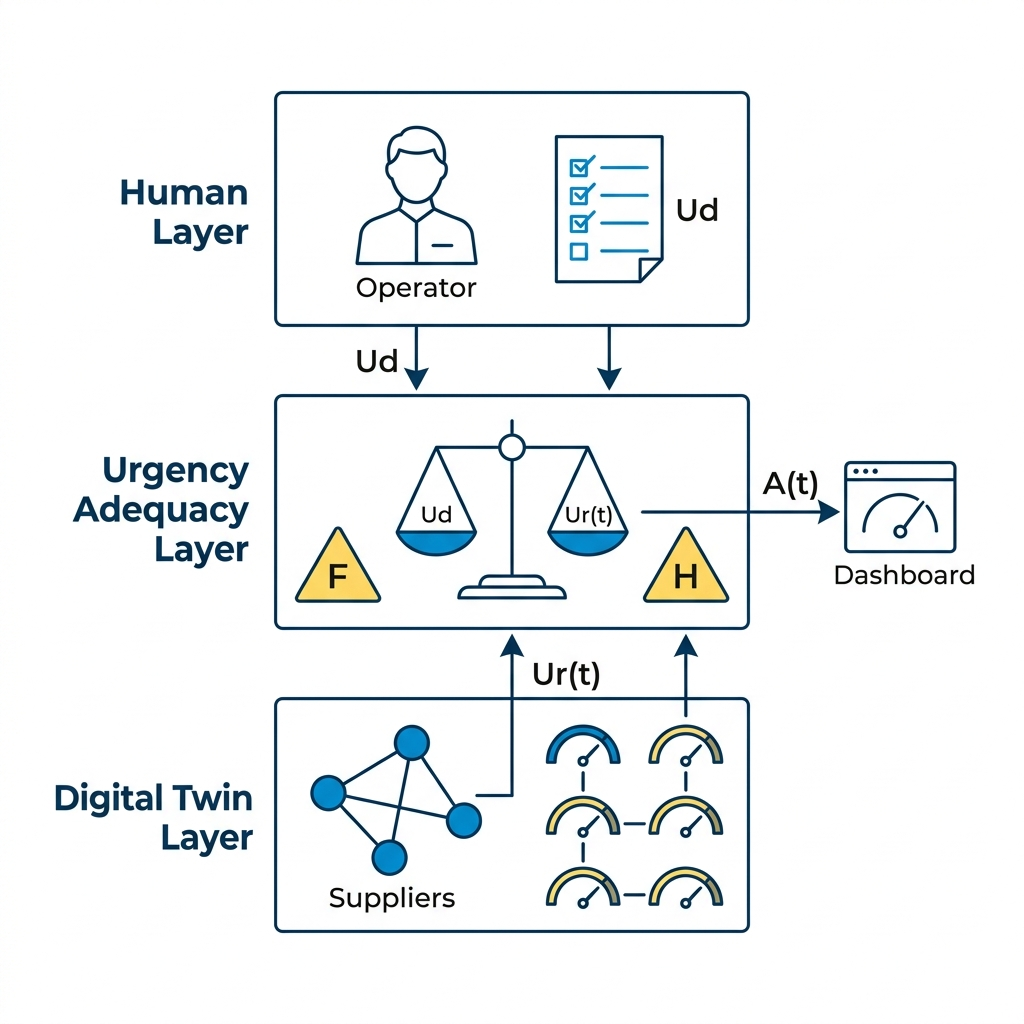
\includegraphics[width=0.85\linewidth]{Images/2.Problem/three_layer_architecture.png}
    \caption{The three-layer urgency adequacy architecture investigated in this work (Challenge~5).}
    \label{fig:todraw_threelayer}
\end{figure}
